\chapter{Les missions}


\section{Missions importantes}
\subsection{Remise en place de l'affiliation}


Ma première mission importante de ce stage a été de remettre en place le système d'affiliation de table du logiciel. L'affiliation est optionnelle et est choisie par le bon vouloir du restaurateur. À mon arrivé côté client voici comment marchait l'affiliation : 

- Un clic long ouvrait sur l'état de la table (sur une table ouverte), un clic simple fermait la table, la table s'ouvrait dès l'instant où un plat était commandé ou choisi.

Et l'objectif de cette mission était de suivre ce schéma d'utilisation :

- Un clic long ferme la table et demande le nombre de convives, un clic simple sur une table ouverte rouvre la table avec l'état. Pour finir la table s'ouvre dès lors que l'on a fait un clic simple sur une table fermée et choisi le nombre de convives.

Pour illustrer mes propos voici des captures d'écrans des deux pages d'affiliation :

\begin{figure}[!htb]
  \centering
  \begin{minipage}[b]{0.45\textwidth}
    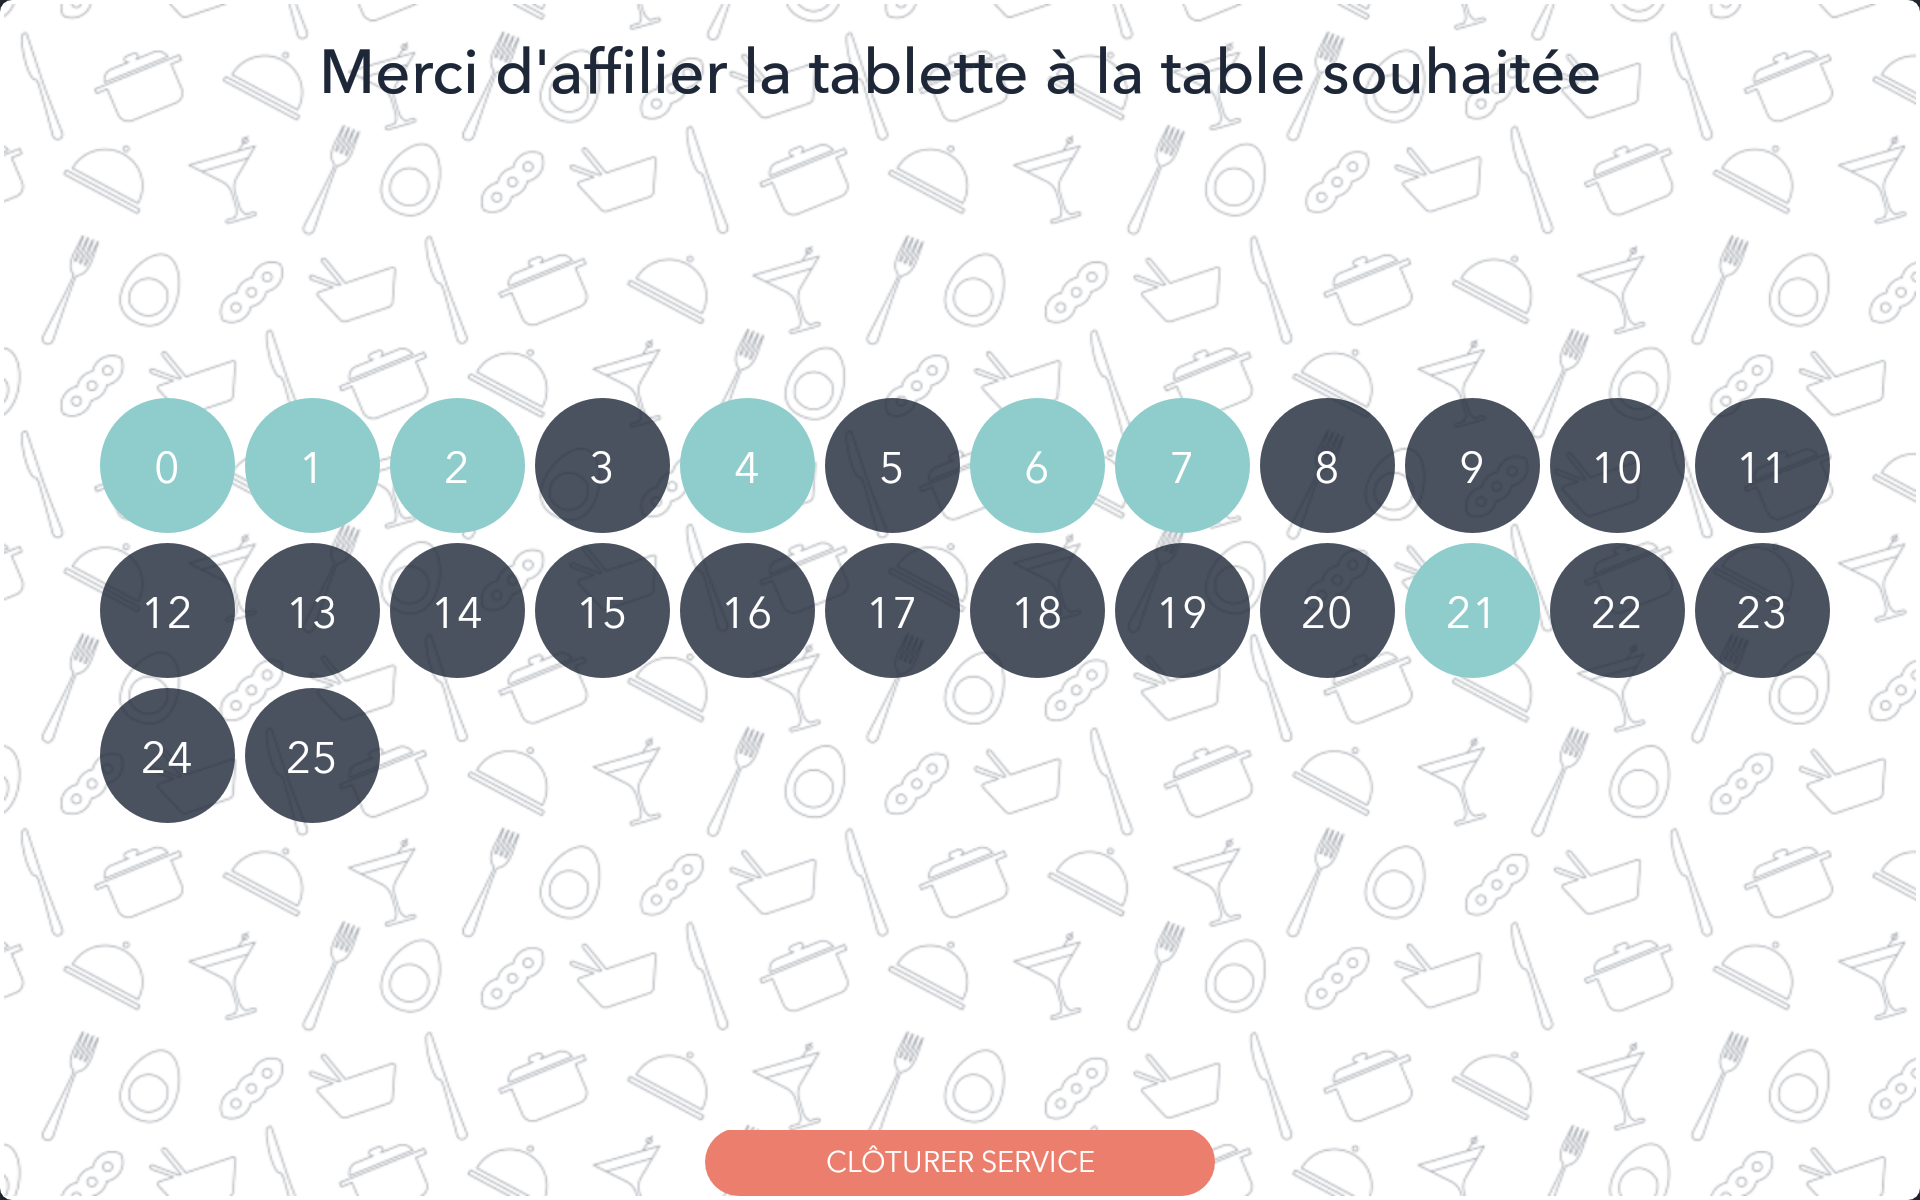
\includegraphics[width=\textwidth]{images/affiliation_table.png}
    \caption{Page d'affiliation de la table}
  \end{minipage}
  \hfill
  \begin{minipage}[b]{0.45\textwidth}
    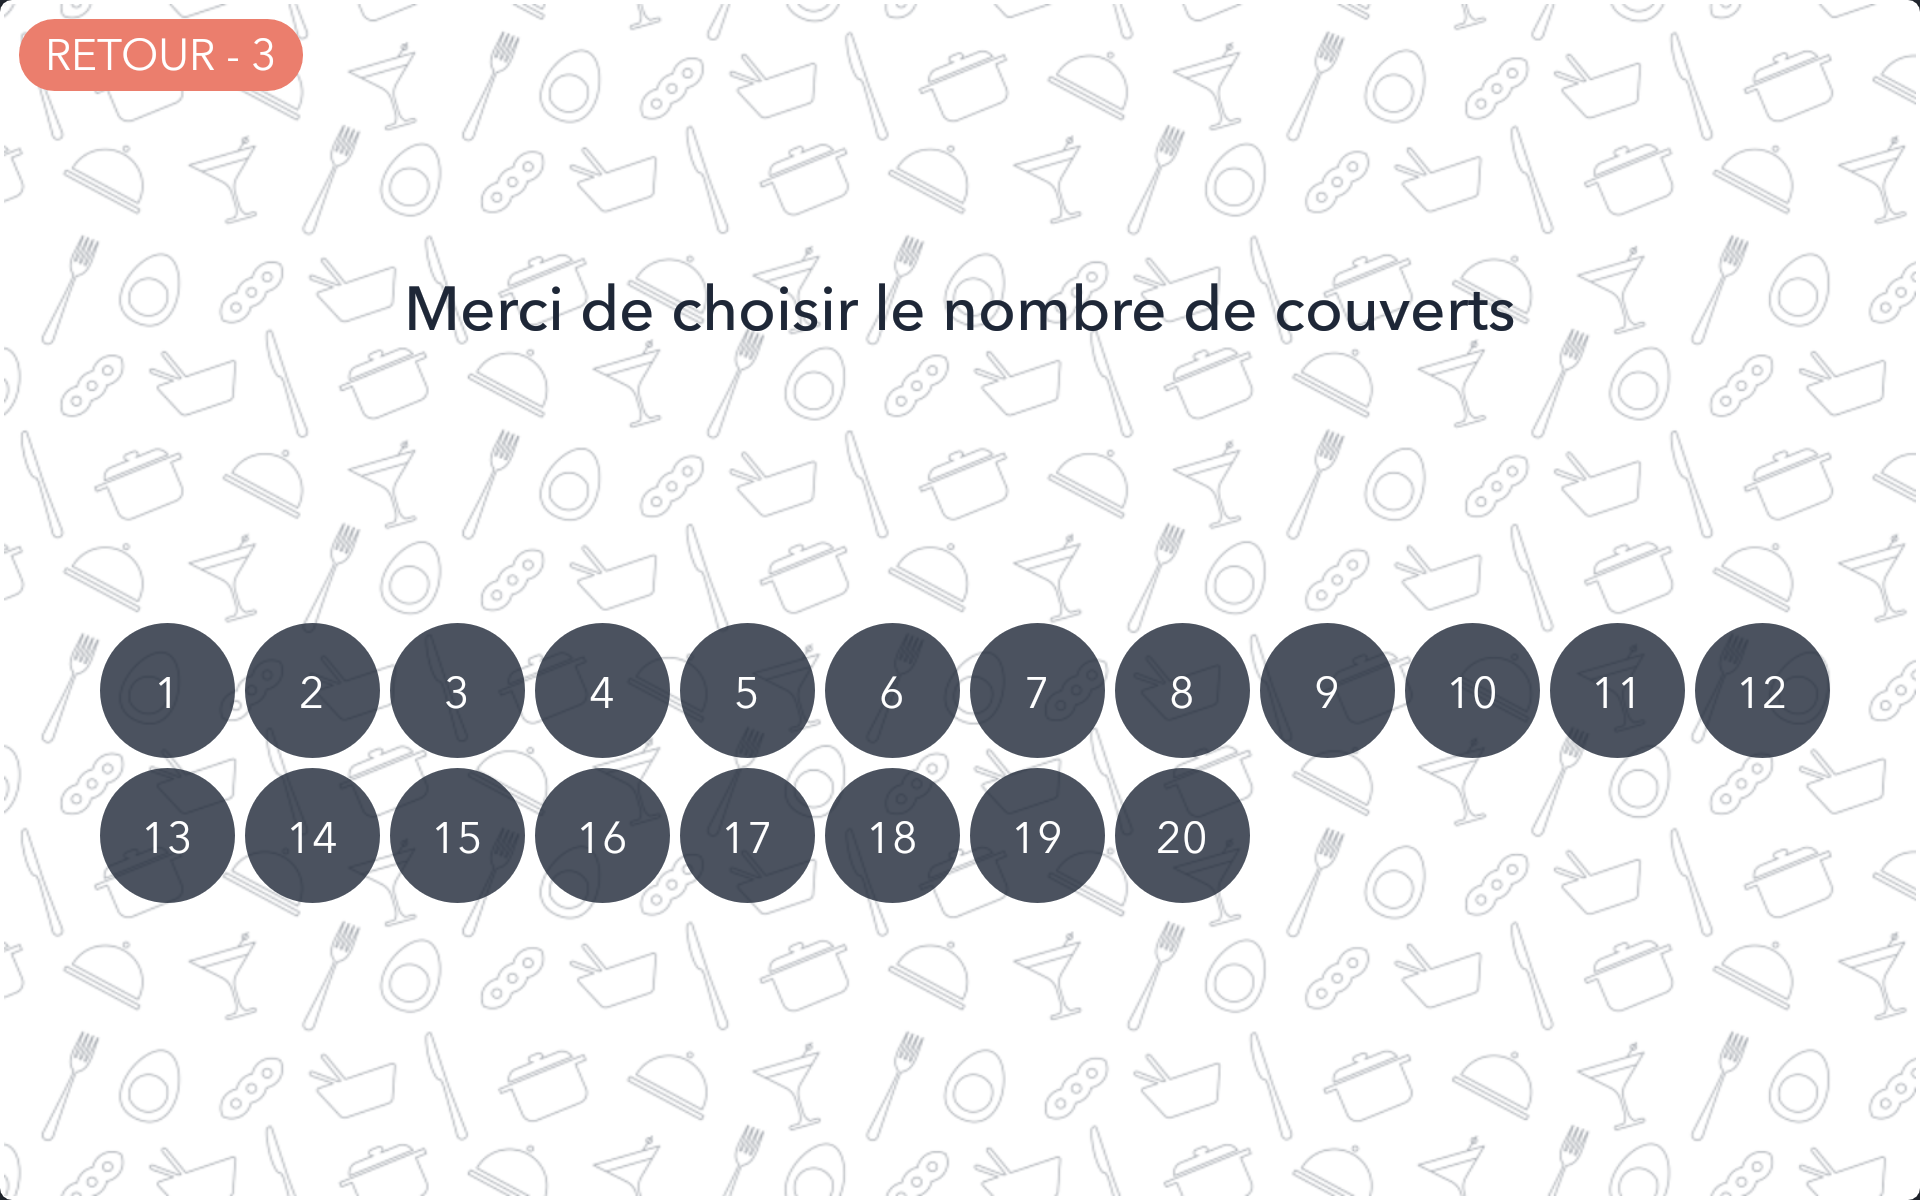
\includegraphics[width=\textwidth]{images/affiliation_convive.png}
    \caption{Choix du nombre de convives}
  \end{minipage}
\end{figure}

Ces deux pages de l'application sont réservées au serveur. C'est lui qui va choisir la table et le nombre de convives. Il a pour cela à sa disposition une liste ou choisir la table dans un premier temps et le nombre de convives dans un deuxième temps. La couleur bleu clair que l'on observe sur certaines tables signifie qu'elles sont ouvertes. C'est sur ces tables que par exemple un clic long entraînerai une fermeture puis une demande du nombre de convives. Les tables sans cette couleur sont donc logiquement des tables fermées.

En plus de cette mission où il a fallu repenser l'affiliation d'un point de vue utilisateur, il m'a été demandé de repenser complètement la structure existante dans l'affiliation. Plus précisément, ma mission consistait à utiliser en Android ce qu'on appelle un "RecyclerView" qui est un conteneur de vues (ici les vues sont les ronds que l'on peut voir dans les captures d'écran ci-dessus). En effet, construire une vue peut être une opération lourde et aujourd'hui Tastycloud commence à avoir des clients qui peuvent par exemple avoir des centaines de tables.

\begin{figure}[!htb]
  \centering
  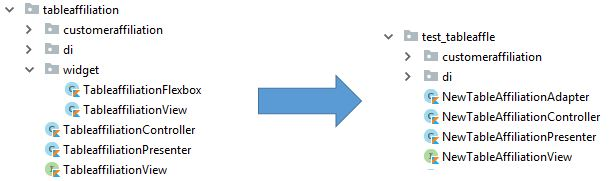
\includegraphics[width=115mm,scale=0.5]{schema_affiliation}
  \caption{Objectif structural de la mission}
  \label{fig:boat1}
\end{figure}

Comme on peut le voir dans la figure ci-dessus à gauche, l'ancienne version possédait une classe "Flexbox" qui utilisait un "FlexboxLayout" qui est donc un outil de mise en page d'Android moins adapté que le "RecyclerView" que je devais moi mettre en place.


Pour le développement de cette structure j'ai donc dû apprendre et réfléchir au fonctionnement du RecyclerView. J'ai dans un premier temps, fais des tests sur la structure déjà existante côté utilisateur, puis j'ai commencé à changer le XML pour mettre en place le ReyclerView. Un premier problème s'est posé quand j'ai compris que je ne devais pas utiliser la même structure qu'avant ce que j'avais fait naïvement dans un premier temps. C'est à dire utiliser un répertoire widget ou j'aurais mis "TableaffiliationRecycler". Après m'être renseigné sur internet et à l'aide de mon tuteur, j'ai compris que le "RecyclerView" a un attribut "adapter". Ce dernier sert à faire la liaison entre le RecyclerView et le contrôleur. Le contrôleur contiendra les logiques précédemment définies à savoir les clics longs et courts et leurs actions ainsi que la création des listes d'éléments qui seront passés à l'adaptateur.

Il a donc fallu créer : 

- Un contrôleur qui contiendra la logique utilisateur et qui créera la liste de tables en fonction de leurs statuts (ouvert, fermé) appelés depuis la base de données de l'application.

- Un adaptateur qui sera en attribut du RecyclerView et qui contiendra la liste des tables.  C'est dans ce dernier que les tables seront traitées une par une pour donner l'effet visuel de table ouverte ou non (rond bleu clair ou non)

- Un presenter qui fera le lien avec la base de données. Ce sera lui qui remontera les informations dans le contrôleur. Le contrôleur héritera d'une interface "View" qui elle contiendra les fonctions appelées par le presenter (en asynchrone).

Bien évidemment, après ce travail de modélisation il faut le réaliser. Heureusement, une structure similaire existait déjà pour une autre fonctionnalité dans l'application, j'ai pu m'en inspirer pour ensuite mettre en place la propre logique de l'affiliation. Seulement, j'ai dû aussi m'inspirer de ce qui existait déjà pour l'affiliation et plusieurs problèmes ont été rencontrés. Le principal a été de convertir toute la logique du Flexbox (donc sur la figure précédente le "TableaffiliationFlexbox") dans le contrôleur.  Ce dernier s'occupait d'ajouter les vues (donc les tables) et de leur attribuer une couleur selon qu'elles étaient ouverte ou non. La première étape à déjà été de construire la liste des tables dans le contrôleur. Pour cela, mon tuteur a décidé de créer une nouvelle table dans la base de données "Table" et d'utiliser un nouveau modèle "TableInformation" qui aura comme attribut le nombre de tables maximum du restaurant et la liste des tables ouvertes (Les éléments de la liste c'est donc par rapport à la nouvelle table créée). Nous avons décidé avec mon tuteur cette solution qui sera beaucoup plus simple pour construire la liste des tables par rapport à ce qui a été fait précédemment pour contrôler ce qui est ouvert ou non. 

Relativement à ce qui a été dit sur le presenter, c'est un cas typique de son utilisation. Lors de l'appel du contrôleur dans l'application une fonction est appelée ("onAttach" dans Android). C'est celle-ci qui est appelée quand le contrôleur est associé à la page courante affichée sur l'application. C'est aussi dans cette dernière que nous allons appeler les fonctions du presenter. Dans notre cas courant voilà ce qui a été fait : Le presenter appelle une fonction dans le OnAttach, ce dernier rappelle une fonction de la vue de manière asynchrone en lui passant un paramètre (donc TableInformation). Cette fonction est définie dans le contrôleur. Le presenter s'occupe lui de faire l'appel à la base de données et à récupérer les informations. Le contrôleur traite TabeInformation dans sa fonction, créé la liste et l'a passe à l'adaptateur. Nous pouvons faire un schéma de ce fonctionnement pour mieux comprendre (un diagramme UML est aussi disponible en annexe).

\clearpage


\begin{figure}[!htp]
  \centering
  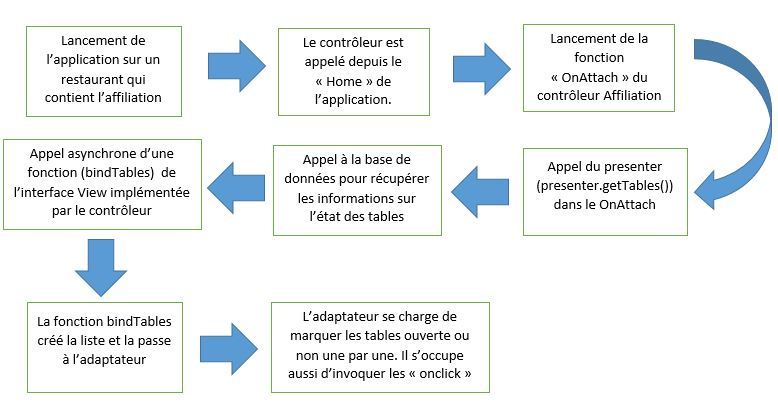
\includegraphics[width=115mm,scale=0.5]{schema2_affiliation}
  \caption{Chemin du programme pour l'affichage des tables}
  \label{fig:boat1}
\end{figure}

Pour ce qui est du presenter il aura des fonctions auxquels nous feront ce qu'on appelle une souscription pour que ce soit asynchrone. Par exemple getTables aura la forme suivante :

\begin{lstlisting}[frame=single]  % Start your code-block
    
    fun getTables() {
        repository.getAllTables()
                .subscribe{ view?.bindTables(it) }
                .toDisposables("getTables")
    }
    
\end{lstlisting}

C'est ainsi que marcheront les appels pour récupérer des informations de la base de données dans le contrôleur. Nous aurons des fonctions définies dans l'interface View qui seront utilisées dans le contrôleur. Le paramètre passé contiendra les informations relatives à la base de données et c'est avec ces informations que nous ferons les traitements.\\

C'est avec l'aide de mon tuteur que j'ai pu comprendre comment créer le chemin pour récupérer les informations et faire le lien avec la base de données. Notamment avec la fonction citée ci-dessus et faire le chemin pour le "repository.getAllTables()". Dans la mise en place de la nouvelle affiliation. Nous avons utilisé cette nouvelle table :

\begin{lstlisting}[frame=single]  % Start your code-block
    
open class TableEntity(
        @PrimaryKey
        override var id: Int = 0,
        open var table_information: String = "",
        open var nb_customers: Int = 0,
        open var is_validated: Boolean = false
) : RealmObject(), Indexed<Int>
    
\end{lstlisting}

TableInformation aura elle une List<Table> des tables ouvertes. Par rapport à l'adaptateur, j'ai suivi ce qui a été fait sur d'autres exemples de l'application j'ai donc entrepris de mettre en place le design pattern "View Holder". Il va construire les vues la première fois et ensuite pourra les mettre à jour sans les reconstruire. C'est ceci qui va permettre à la construction de la liste d'être moins lourde. C'est dans ce ViewHolder que seront faites les mises à jour de couleurs, de texte et dans lequel seront invoqués les "onclick". La logique donnée en début de partie sera par contre définie dans le contrôleur. 

\clearpage

Une fois tout ceci mis en place, il a fallu appliquer la même logique pour les convives. Une fois la méthode assimilée sur l'affiliation le travail sur les convives a été plus rapide. Il a fallu instaurer la même logique avec un adaptateur, un contrôleur et un presenter. Contrairement à l'affiliation les vues doivent simplement amener sur le "home" de l'application quand on clic dessus. La construction de la liste est définie par un nombre X de convives maximum et ainsi une liste de X vues sont créées. Nous n'avons pas besoin d'appel à la base de données dans ce cas le nombre est défini autrement.

Si nous pouvons parler de cette mission d'un point de vue graphique, j'ai aussi géré le cas ou le nombre de tables dépasse le cadre donné au RecyclerView. On peut alors dans ce cas tout simplement scroller. Auparavant nous avions un bug graphique et les ronds prenaient tout l'écran. J'ai dû pour cela me renseigner sur les logiques arborescentes d'Android en XML et j'ai donné différents poids aux éléments graphiques : 

\begin{figure}[!htp]
  \centering
  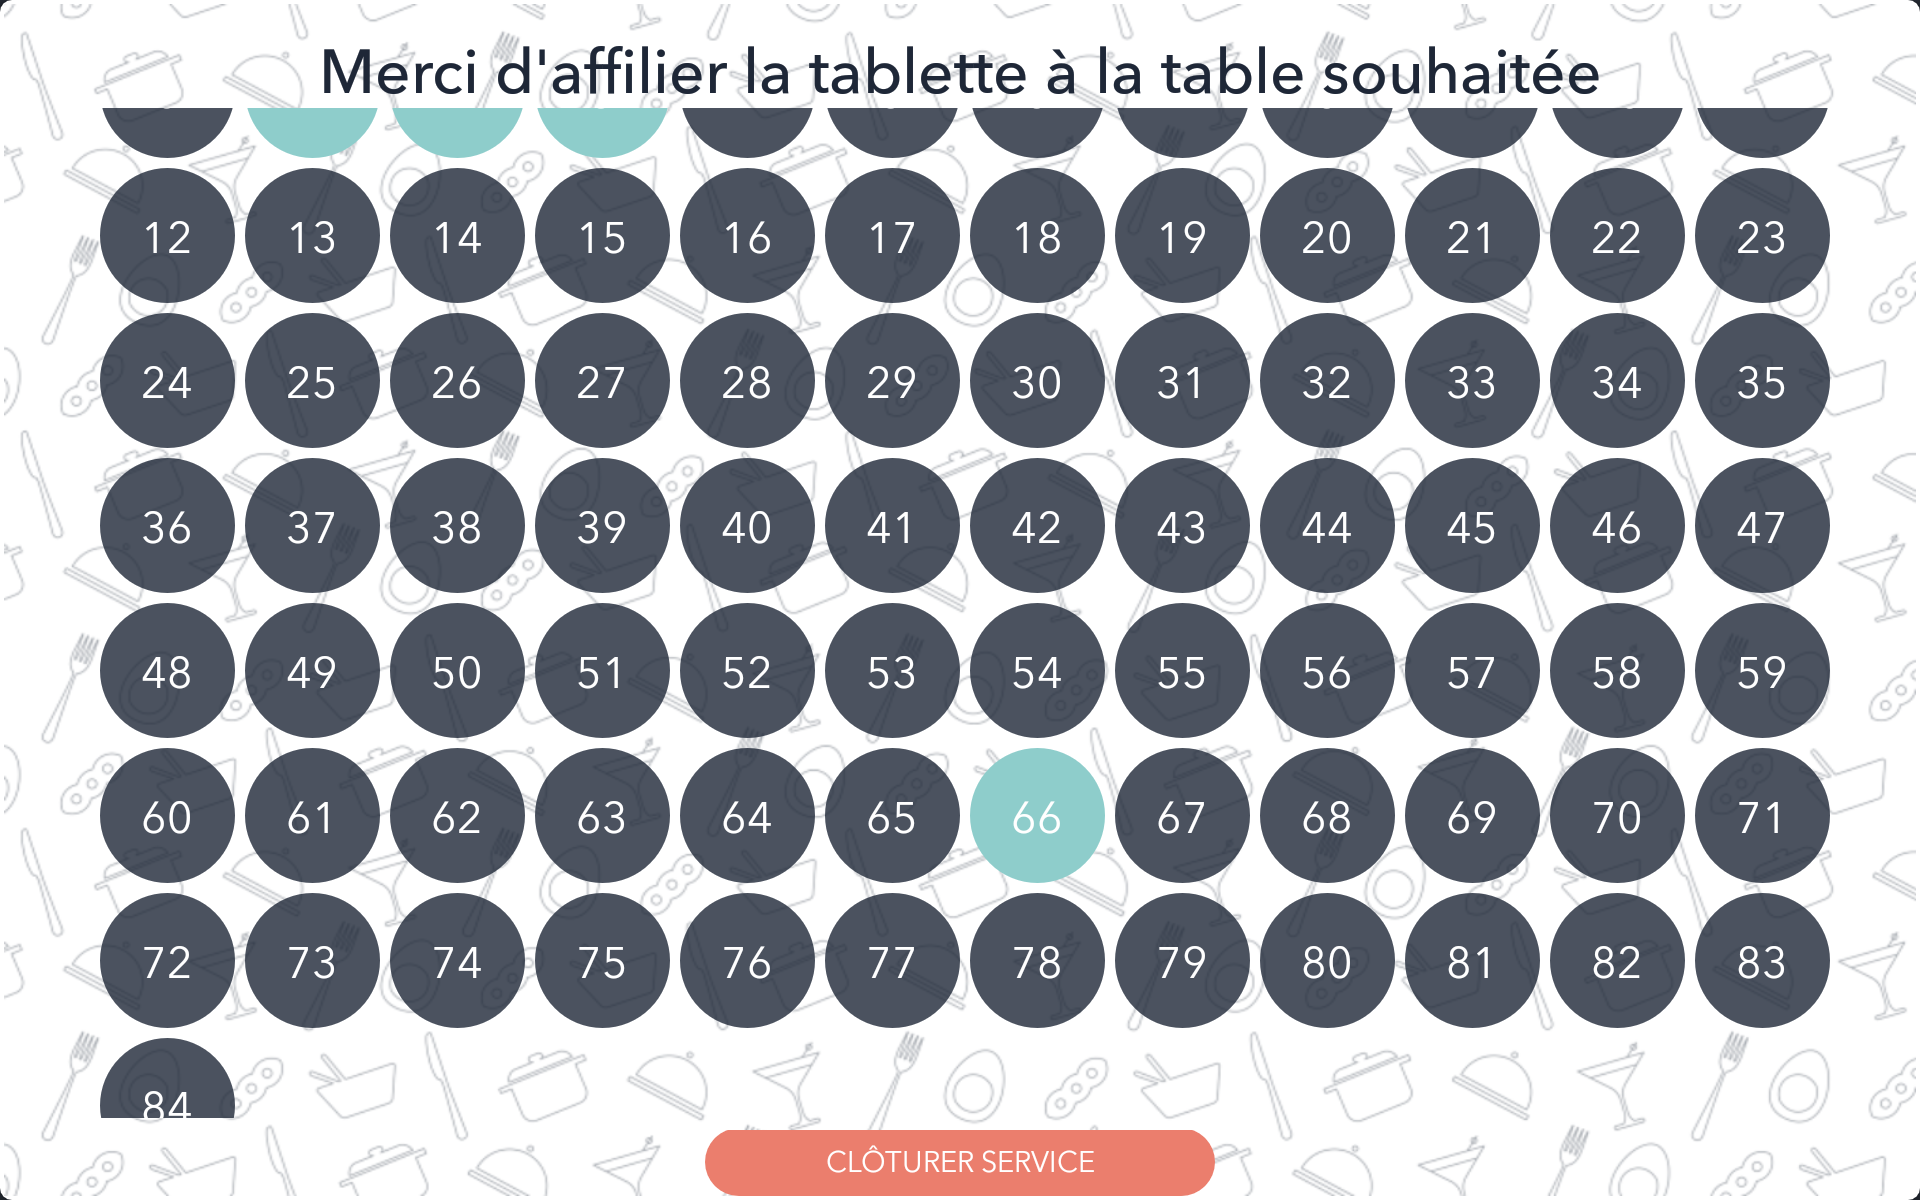
\includegraphics[width=115mm,scale=0.5]{images/affiliation_screen.png}
  \caption{Exemple de restaurant ou le nombre de tables est élevé}
  \label{fig:boat1}
\end{figure}

Comme on peut le voir sur cette capture d'écran, nous pouvons découper la page en 3 vues : Le titre en haut, le RecyclerView (donc le conteneur) et enfin le bouton pour clôturer le service. Pour avoir ce résultat j'ai décidé de donner au conteneur des 3 vues un poids avec l'attribut "WeightSum" et de donner 9/10ème de ce poids au RecyclerView.

Cette mission a surtout été une mission de recherche et d'adaptation d'un modèle à l'autre. La conception et le développement y étaient relativement restreints mais elle m'a permis de bien comprendre comment fonctionne l'application d'un point de vue technique. Elle m'a également permis de bien comprendre certaines subtilités d'Android. C'était la mission la plus technique du stage car très peu visuelle par rapport aux autres. Ce qui n'est pas le cas, par exemple, de la mission suivante où le développement s'est fait de zéro et où il a fallu inventer une nouvelle structure.

\clearpage

\subsection{Tutoriel}

Dès mon entretien l'équipe m'avait parlé d'un projet de didacticiel à mettre en place sur le logiciel visant les personnes moins à l'aise avec la technologie pour leur proposer un parcours ludique qui expliquerait rapidement un chemin d'utilisation de l'application de manière visuelle. Avant mon arrivée, l'équipe a réfléchi aux différentes pop-ups présentes dans le tutoriel et a demandé à des designers de mettre en place une première version sous forme de PNG :

\begin{figure}[!htb]
  \centering
  \begin{minipage}[b]{0.45\textwidth}
    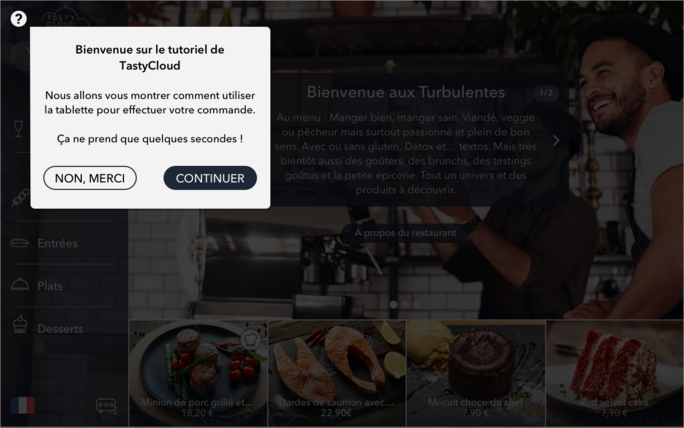
\includegraphics[width=\textwidth]{images/tutoriel_design.png}
    \caption{Première étape du didacticiel}
  \end{minipage}
  \hfill
  \begin{minipage}[b]{0.45\textwidth}
    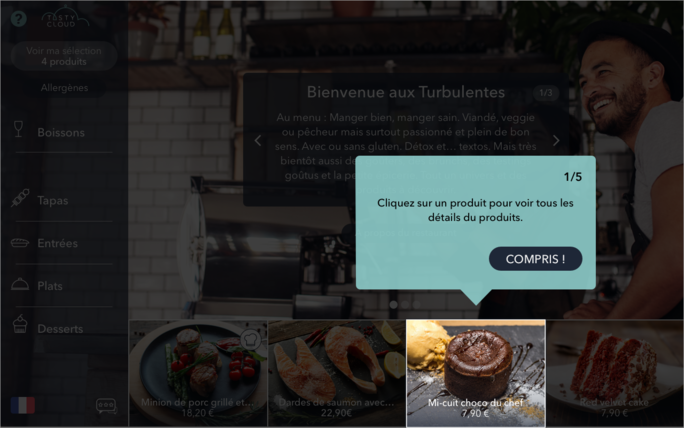
\includegraphics[width=\textwidth]{images/tutoriel_design2.png}
    \caption{Deuxième étape du diacticiel}
  \end{minipage}
\end{figure}

Comme on peut le voir sur les images ci-dessus, le but était de travailler avec des pop-ups et de parcourir l'application. J'avais à ma disposition ces 2 images et les textes à mettre dans les pop-ups pour les étapes suivantes. Le didacticiel étant un nouveau projet j'ai dû dans un premier temps faire des recherches sur quoi utiliser pour mettre en oeuvre une première version. J'ai d'abord décidé de mettre en place le bouton sur la page d'accueil de l'application entre le bord gauche et le logo. Tout ceci se fait dans le XML, j'ai centré le bouton dans l'espace vide entre le logo et le bord gauche. Après cette première étape terminée il a fallu trouver un moyen de créer les pop-ups. J'ai d'abord réfléchi au "DialogBox" d'Android. Cet outil affiche par défaut une fenêtre avec deux boutons "Ok" et "Annuler" et grise le fond. Je me suis vite rendu compte que cet outil n'était pas vraiment fait pour l'utilisation d'un didacticiel car il aurait fallu redéfinir tout le contexte par défaut. Les DialogBox sont plus utiles pour un cas où l'on aura un pop-up qui nous demanderait de cocher des choix ou bien entrer un texte pour un traitement futur ce qui n'était pas réellement le cas d'utilisation ici. Après recherche sur le guide de développeur d'Android je me suis aperçu qu'un autre outil "PopupWinow" répondait plus à mes attentes. Dans le cas du didacticiel nous avons besoin que la pop-up s'affiche, s'efface et se réaffiche assez souvent sans avoir de ralentissement. Avec un DialogBox cela aurait été moins fluide. Le PopupWindow était intéressant car il permet facilement le changement de position (les pop-ups du didacticiel changent de place assez souvent). On peut aussi facilement lui associer un layout (donc une page graphique) dans le XML.

J'ai donc dans un premier temps créé mon layout en XML en reprenant les PNG que l'on m'avait fournis ci-dessus. On a par ailleurs décidé avec mon tuteur qu'il serait mieux de donner la possibilité à l'utilisateur de pouvoir quitter le tutoriel à tout moment. Par conséquent, excepté pour le message d'introduction qui propose déjà un bouton pour quitter, nous avons décidé de mettre un bouton en haut à gauche pour quitter durant les autres étapes du tutoriel. Il a aussi été décidé à ce moment-là de garder la même couleur pour tout le tutoriel et de ne plus utiliser le bleu que l'on peut apercevoir dans la deuxième capture d'écran ci-dessus.

D'un point de vue graphique nous avons donc 3 principaux conteneurs dans le XML du pop-up. Le premier en haut et horizontal qui contient le bouton pour quitter et le compteur pour savoir à quelle étape on est, le deuxième qui contient le texte (titre et texte) qui est vertical et le dernier qui contient les deux boutons.

\clearpage


\begin{figure}[!htp]
  \centering
  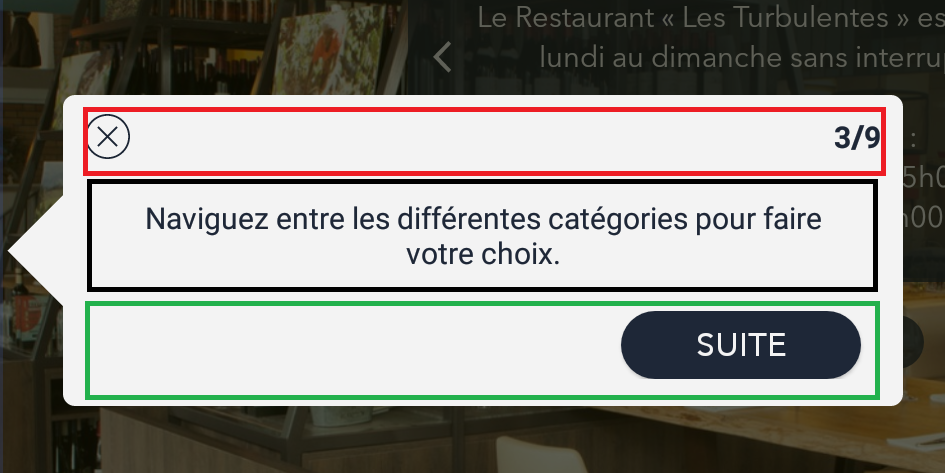
\includegraphics[width=115mm,scale=0.5]{images/tutorial_popup.png}
  \caption{Exemple d'une étape du didacticiel}
  \label{fig:boat1}
\end{figure}

Nous avons par exemple dans l'image ci-dessus décomposé le didacticiel en 3 rectangles qui délimitent les conteneurs définis précédemment. Ce qu'on peut noter c'est que dans certains cas certains éléments graphiques seront rendus invisibles. Par exemple, tout rectangle rouge dans le message de bienvenue du didacticiel est caché. Dans les étapes du tutoriel c'est le titre présent dans le rectangle noir qui est caché et le bouton de gauche dans le rectangle vert.

Une dernière étape dans la mise en place graphique des pop-ups ont été les triangles. On peut dans la capture d'écran en voir un à gauche. Ces triangles peuvent être présents en haut, en bas, à droite, à gauche. J'ai au début pensé à définir un triangle que je pourrais déplacer et retourner en fonction des cas. Cependant c'était une solution loin d'être pratique surtout que l'on peut dans le futur rajouter des étapes. J'ai donc directement défini 4 triangles dans le XML qui se mettaient à chaque fois dans la bonne orientation et au milieu d'un des quatre côtés. Ces quatre triangles sont donc cachés et peuvent être rendus visibles dans le code. C'est une utilisation bien plus simple par rapport à ce que j'avais préconisé dans un premier temps, c'est aussi bien plus simple de réutilisation.

Une fois le côté graphique des pop-ups créé, il a fallu penser à la réutilisabilité du didacticiel. C'est à dire prévoir les cas où il faudrait rajouter des étapes, changer le style graphique etc. Pour cela j'ai décidé de définir ma propre classe qui hérite de PopupWindow et qui aura en attribut les textes, les boutons et les triangles. J'ai pensé à un système où l'on aurait seulement besoin de définir les textes, le nombre d'étapes et les localisations des pop-up sur l'écran pour créer le tutoriel. Pour revenir sur les triangles j'ai par exemple une fonction de cette classe héritée "setTriangle" qui prend en paramètre une "Orientation" soit une énumération qui peut prendre comme valeurs différentes : LEFT, BOTTOM, TOP, RIGHT, GONE. Pour les positions différentes et pour le cas où il n'y a pas de triangles. Cette fonction est simplement appelée selon les différentes étapes et selon l'orientation que l'on souhaite. Cette solution permet par exemple une lecture du code simple si quelqu'un devait reprendre mon travail dans le futur. J'ai aussi pensé à créer deux fonctions, une "startTutorial" qui permet de lancer les éléments graphiques du tutoriel (c'est à dire après avoir appuyé sur "continuer" sur la première pop-up) et une autre fonction "nextStep" qui permet l'incrémentation du compteur, du texte et de la position de la pop-up. Ces 3 éléments étant définis dans des tableaux à l'initialisation.

Une fois que cette première étape a été réalisée j'ai été confronté à un premier problème auquel il a été, dans un premier temps, difficile de répondre. Comme on peut le voir dans les captures d'écrans de la page précédente, pendant que le didacticiel est déroulé le fond de l'application est foncé et les éléments sur lesquels on doit mettre l'accent (par exemple le bouton du tutoriel et un des plats de la barre de suggestion) sont mis, eux, en transparent.

Dans un premier temps il a fallu mettre le fond en foncé. J'ai alors fait des tests sur l'élément qui englobait tous les autres dans la page d'accueil de l'application. Le problème est que cet élément étant parent d'autres éléments fils, changer la couleur de fond ne se verra pas, en effet ses fils vont "prendre le dessus". J'ai alors testé avec l'attribut "foreground" que l'on pourrait traduire par premier plan. Dans ce cas le fond devenait bien foncé mais malheureusement on a fait face au problème que les éléments graphiques ajoutés seront forcément sous le premier plan et donc tous les éléments seront assombris. Il a donc été décidé de faire une nouvelle arborescence. On va dans un premier temps définir un père qui aura un fils qui lui va contenir tous les éléments graphiques de la page d'accueil. Hors de ce fils, on va définir une nouvelle vue qui prendra l'ensemble de la page et qui sera "au dessus" de l'autre vue qui contient tous les autres éléments graphiques. Ainsi sur cette vue on pourra définir les pop-ups et les éléments à rendre plus clair. On peut donner un aperçu de cette arborescence avec le code XML ci-dessous : 

\begin{lstlisting}[frame=single]  % Start your code-block
    
<RelativeLayout
    android:id="@+id/home"
    android:layout_width="match_parent"
    android:layout_height="match_parent">
    
    <FrameLayout... />
    
    <com.tastycloud.ui.home.tutorial.BrightView.../>
    
    </RelativeLayout>
    
\end{lstlisting}

Le RelativeLayout est le père, le FrameLayout contient tous les éléments graphiques de la page et le BrightView sera celui qu'on affichera quand on lancera le didacticiel. Rendre les éléments plus clairs a été un autre problème, il a fallu réfléchir à une solution pour rendre le fond foncé sauf à quelques endroits précis où il devait devenir transparent. J'ai pensé dans un premier temps à créer au dessus du BrightView un "ImageView" (un élément graphique pour les images) et à superposer cet élément sur ceux qu'il fallait rendre plus clair. Seulement, cette solution n'est pas vraiment viable car il faudrait reprendre le même "design" qui existe déjà sur les éléments à rendre plus clair pour pouvoir y mettre l'ImageView. On a donc réfléchi à une solution avec mon tuteur et j'ai après quelques recherches sur internet trouvé un moyen de dessiner des formes (rectangle, rond) à l'intérieur de la "BrightView". Ces formes seraient alors transparentes. Comme on peut le voir dans l'extrait de code "BrightView" est une classe définie dans le projet. Elle hérite de FrameLayout et on va alors pouvoir redéfinir sa fonction onDraw. La fonction "onDraw" va contenir elle comme paramètre un "Canvas" qui lui va contenir les appels qui vont permettre de dessiner sur le BrightView. L'idée est d'ensuite avoir ce BrightView en attribut du PopupWindow défini lui aussi dans le code. Ainsi, on pourra directement définir avec cette classe qui étend de PopupWindow les éléments à éclairer, la forme qu'ils doivent avoir, leur emplacement etc... Pour que l'utilisateur ne passe pas par BrightView toutes les fonctions de BrightView pour dessiner des formes (par exemple "setRoundedRectangle", "setRectangle", "setCircle") sont redéléguées à BrightView dans PopupTutorial (donc la classe qui hérite de PopupWindow). C'est à dire qu'on aura des fonctions de ce type dans PopupTutorial :

\begin{lstlisting}[frame=single]  % Start your code-block
    
    fun setBrightViewRectangle(v: View) {
        brightView.setRectangle(v)
    }
    
    fun setBrightViewCircle(x: Float, y: Float, radius: Float) {
        brightView.setCircle(x, y, radius)
    }
    
\end{lstlisting}

Tout ceci est donc fait dans un souci de réutilisabilité et pour que si un autre utilisateur venait à reprendre ce code, qu'il n'est pas à instancier différents éléments pour par exemple créer une nouvelle étape. Les fonctions définies dans BrightView s'occupent d'affecter les valeurs passées en paramètre puis d'appeler le onDraw qui va dessiner l'élément selon le type défini par une énumération et qui est affecté dans les dites fonctions : 

\begin{lstlisting}[frame=single]  % Start your code-block
    
    override fun onDraw(canvas: Canvas?) {
        
        canvas?.drawColor(mTutorialColor); //couleur de fond
        
        //dessine selon de type (DrawType)
        if (mCx >= 0 && mCy >= 0) {
            when (currentDrawType) {
                DrawType.CIRCLE -> canvas?.drawCircle(...)
                DrawType.RECTANGLE -> canvas?.drawRect(...)
                DrawType.ROUND_RECTANGLE -> canvas?.drawRoundRect(...)
                DrawType.EXTRA_RECTANGLE -> {
                    canvas?.drawRect(...)
                    canvas?.drawRect(...)
                }
            }
        }

    }
    
\end{lstlisting}

Comme nous pouvons le voir, on utilise une énumération "DrawType" qui selon les cas va dessiner différentes choses. Soit comme on peut le voir CIRCLE, RECTAGLE, ROUNDRECTANGLE (un rectangle avec les bords rond) et EXTRARECTANGLE (2  rectangles).
Pour que tout ceci soit plus clair nous pouvons faire un diagramme UML de la structure du didacticiel comprenant toutes les classes précédemment définies et les liens entre elles.


\begin{figure}[!htp]
  \centering
  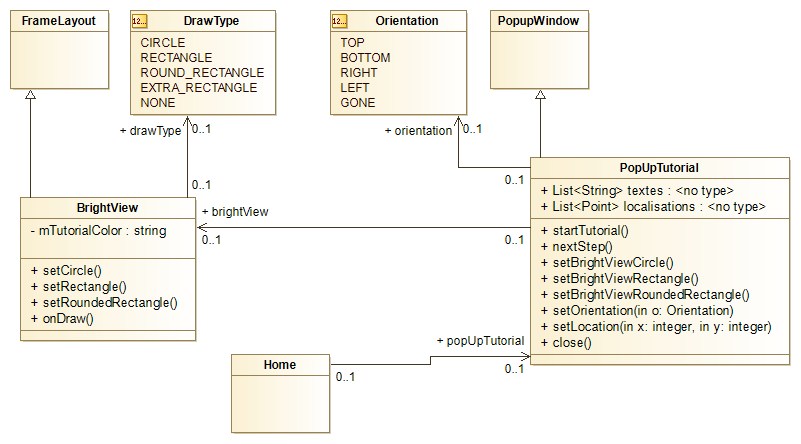
\includegraphics[width=115mm,scale=0.5]{images/diagramme.png}
  \caption{Diagramme UML simplifié du didacticiel}
  \label{fig:boat1}
\end{figure}

Le diagramme est volontairement simplifié pour faire apparaître l'essentiel sur la structure qui a été définie tout au long de cette partie. Home correspond au contrôleur de la page d'accueil où est appelé PopUpTutorial. Il n'est pas nécessaire de connaître les valeurs passées aux fonctions dans la plupart des cas, l'important ici est juste de comprendre la structure globale du didacticiel.

Une fois tout ceci mis en place on peut dorénavant dérouler un tutoriel avec les différentes étapes. Dans la version qui a été définie par Tastycloud le didacticiel comportait 9 étapes (ou 8 selon les cas de restaurants). Ces étapes sont disponibles en annexe. Ce qu'il faut savoir c'est que certaines de ces étapes nécessitent de simuler une navigation et donc de parcourir l'application. Pour un cas unique de restaurant on peut facilement définir un chemin (et c'est d'ailleurs ce qui a été fait dans un premier temps). Cependant, comme dit précédemment, chaque restaurant a ses spécificités. Par exemple certains restaurants ne possèdent pas les allergènes, certains n'ont pas les même structure dans le menu de gauche. Il faut donc adapter tout ceci pour que le didacticiel couvre le plus de cas possible. Un exemple a été pour l'étape où l'on présente la page de sélection de produits. Dans certains cas le menu est différent. 

\begin{figure}[!htb]
  \centering
  \begin{minipage}[b]{0.45\textwidth}
    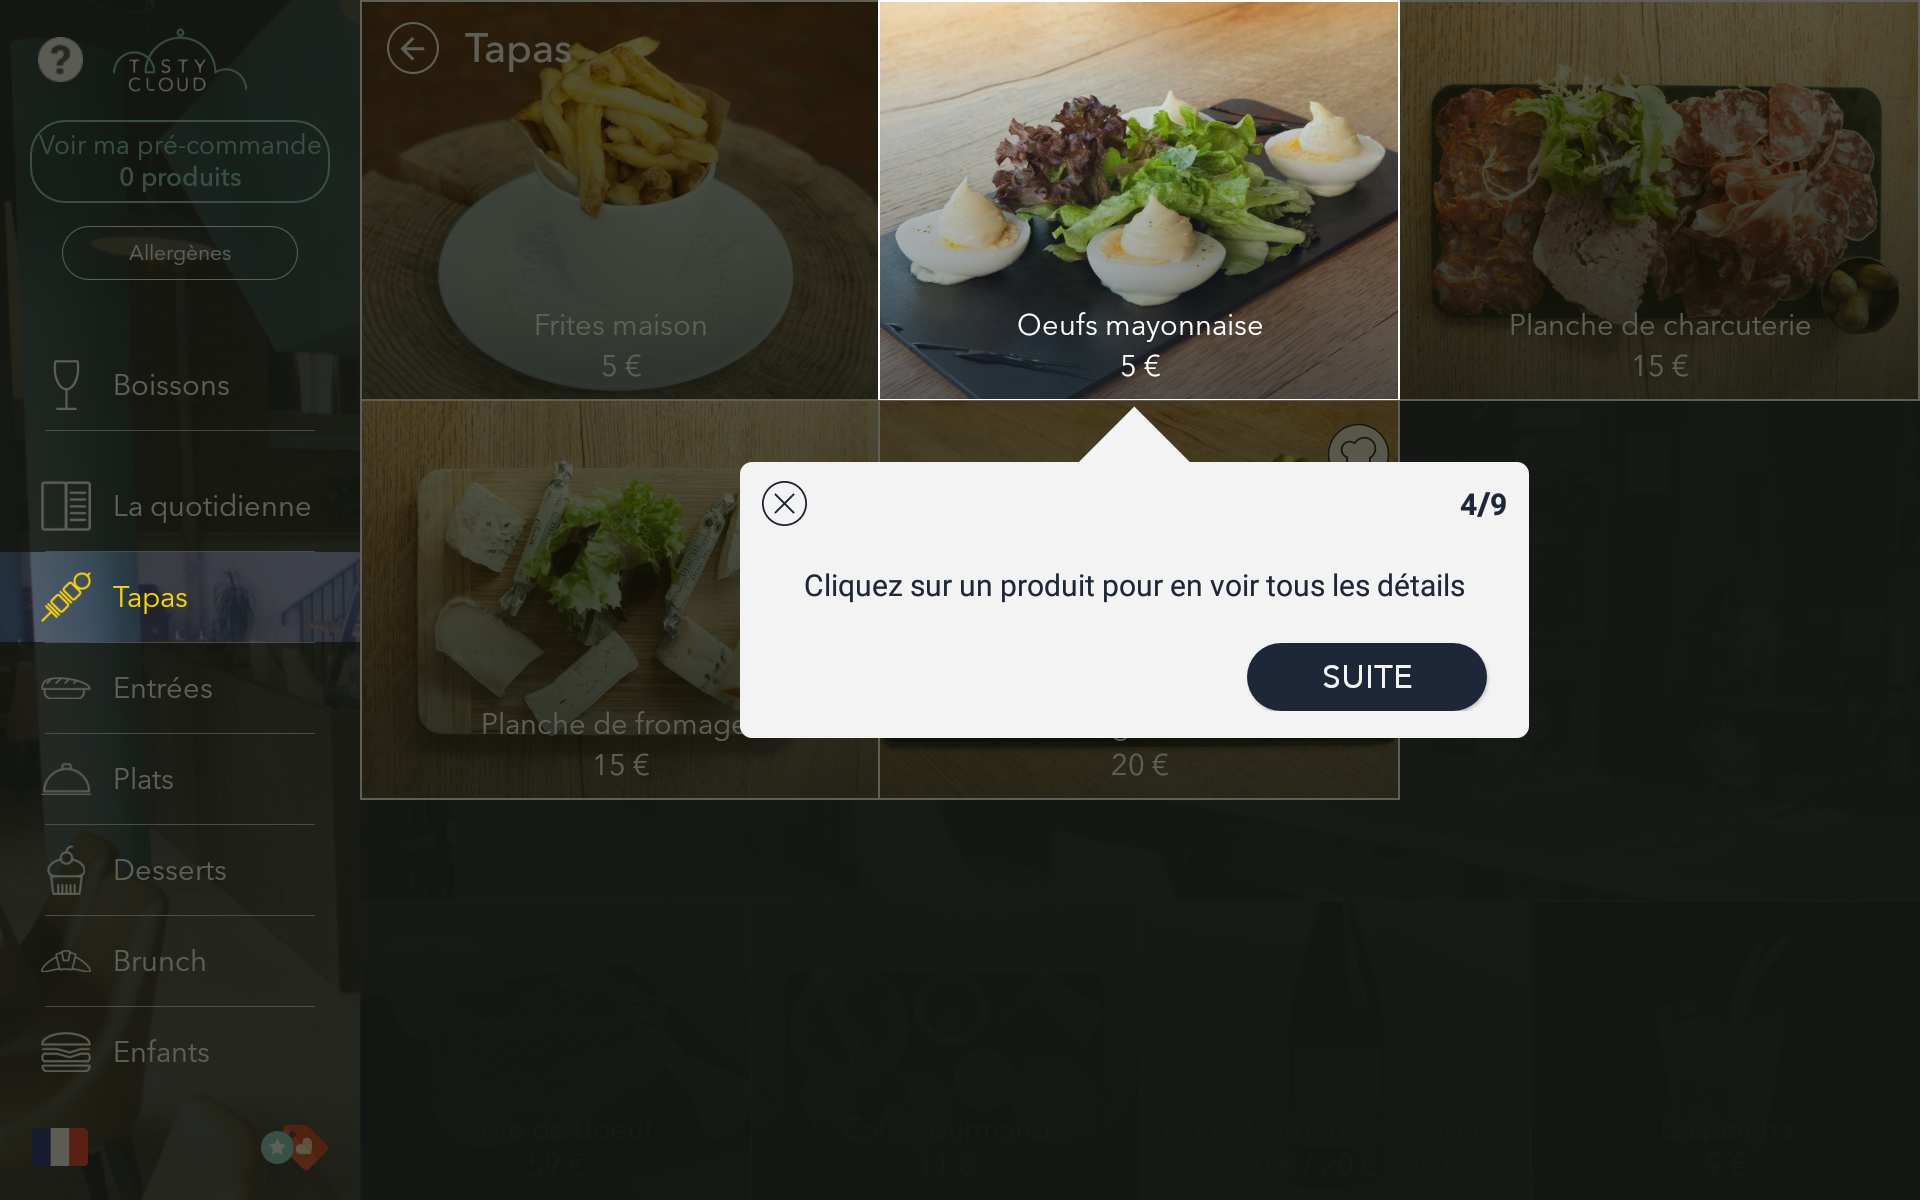
\includegraphics[width=\textwidth]{images/tutoriel_screen2.png}
    \caption{Étape 4 du didacticiel}
  \end{minipage}
  \hfill
  \begin{minipage}[b]{0.45\textwidth}
    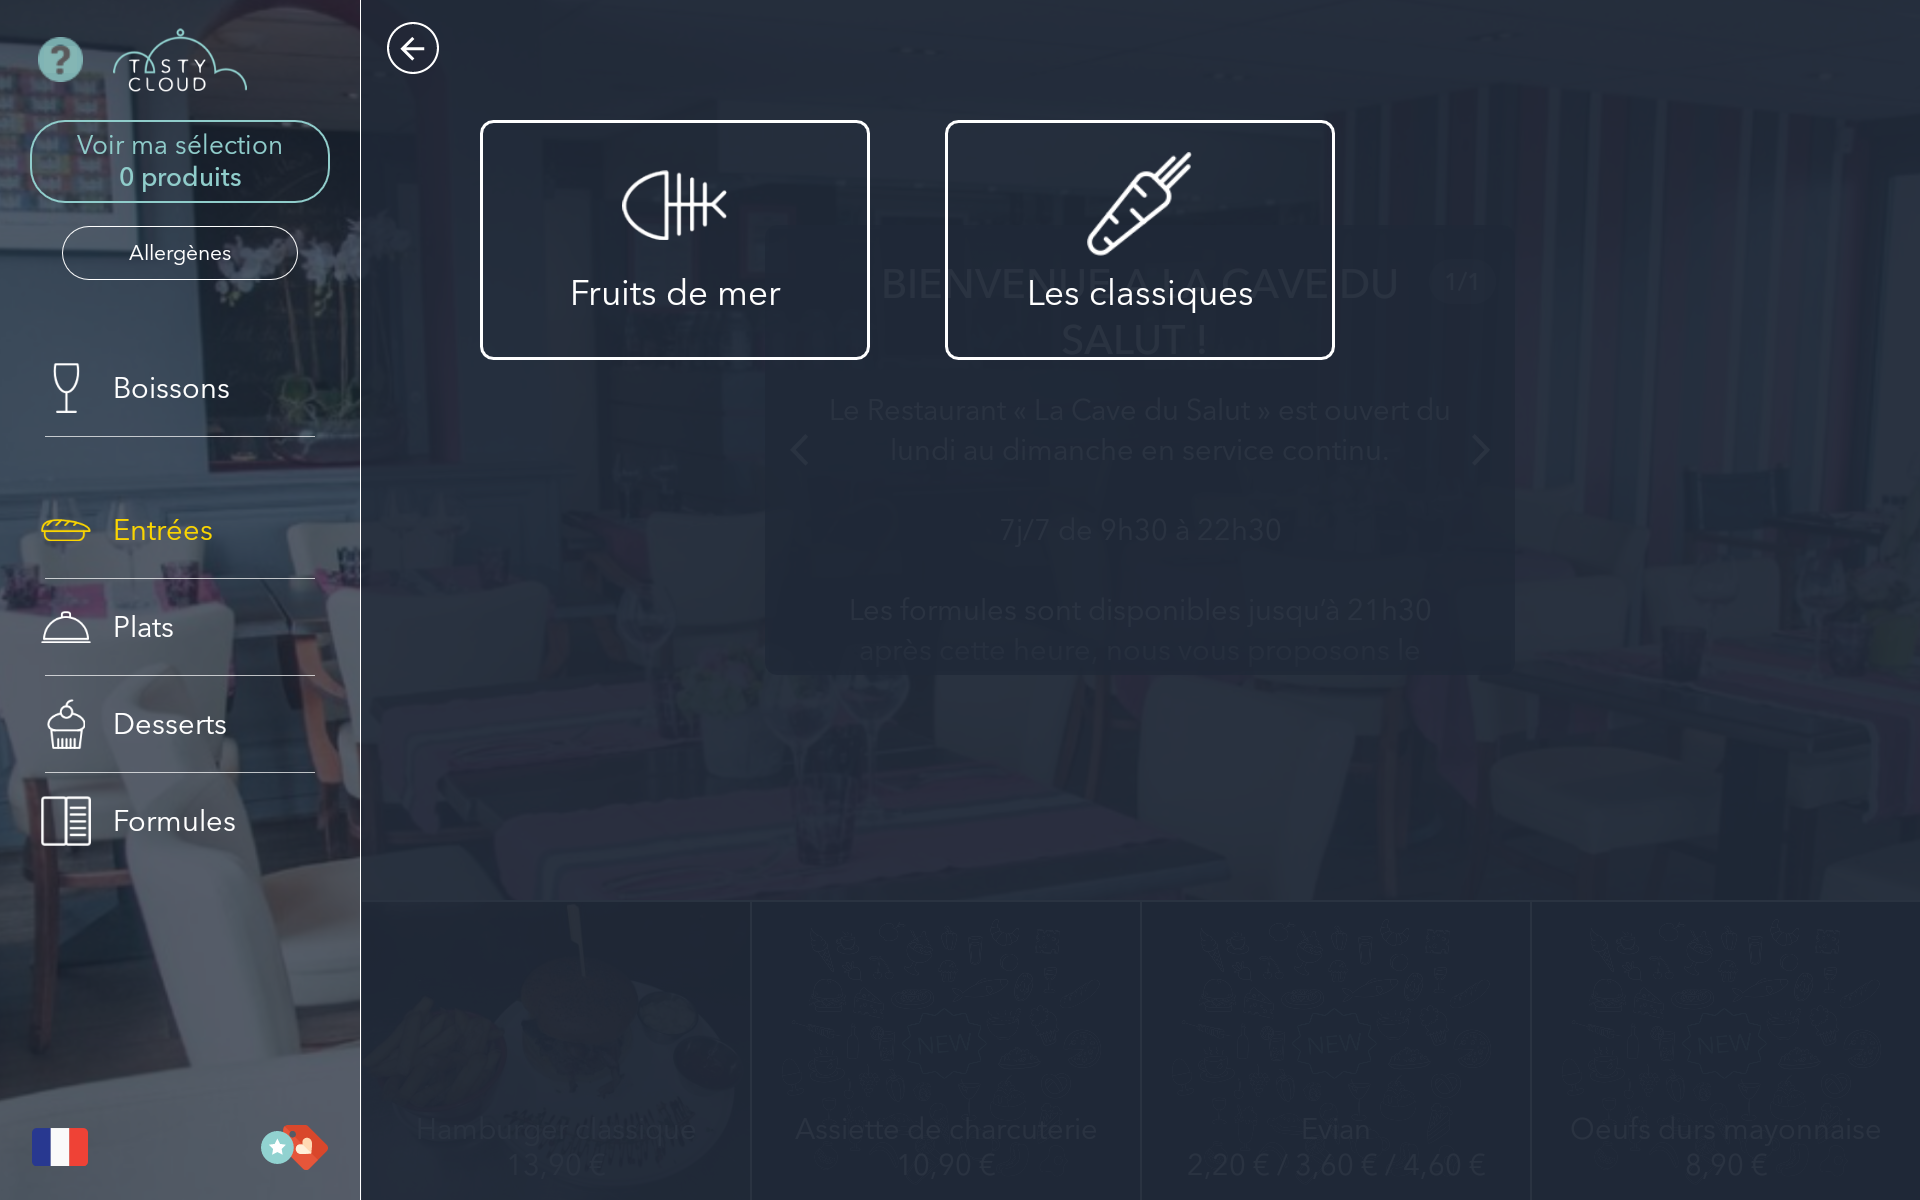
\includegraphics[width=\textwidth]{images/tutoriel_screen1.png}
    \caption{Menu entrées}
  \end{minipage}
\end{figure}

Comme on peut le voir sur les captures d'écrans, il y a parfois un autre menu avant d'atteindre la sélection des produits. Il a fallu, dans le code vérifier ce cas et l'ignorer pour contourner ce problème. Il faut aussi gérer la présence ou non des allergènes. Heureusement le restaurant courant et ses options peuvent être récupérés depuis le home et ces cas particuliers peuvent être traité plus facilement.

Un autre problème a été que le tutoriel nous montre aussi comment commander et comment voir sa sélection. Il a donc fallu simuler un choix et l'afficher dans l'onglet des commandes. Seulement, lorsque l'on mémorise un choix dans l'application celui-ci est envoyé à la base de données. Or, logiquement dans notre cas le didacticiel est juste là pour montrer le fonctionnement de l'application et non pas pour faire des appels à la base. Pour faire face à ce problème j'ai décidé de créer une variable associée au restaurant qui est disponible dans les classes de sélection de l'application et qui permet de faire un test (donc avec cette variable qui est un booléen) pour savoir si oui ou non il faut faire un appel à la base. Dans un premier temps, il n'était même pas prévu de simuler l'utilisation de l'application avec un produit mais finalement lors du développement du tutoriel nous avons trouvé cela plus logique. 

Par exemple, dans la capture d'écran que l'on a sur la page suivante, "les frites maison" sont ajoutées dans la sélection mais elles ne le sont pas dans la base données. C'est à dire qu'elles sont ajoutées seulement graphiquement sur l'application. Dans le cas où l'utilisateur quitte le tutoriel à cette étape, l'élément ajouté "virtuellement" dans la sélection est supprimé. Et seulement celui-là si l'utilisateur avait déjà choisi des produits avant de lancer le tutoriel. Rajoutons aussi que lorsque l'on appui sur le bouton quitter l'application revient toujours sur le menu home, et si on clic sur le didacticiel dans un sous menu, le tutoriel commencera toujours aussi sur le home (sinon le parcours ne se ferait pas sur les bonnes pages de l'application).

\clearpage

\begin{figure}[!htb]
  \centering
  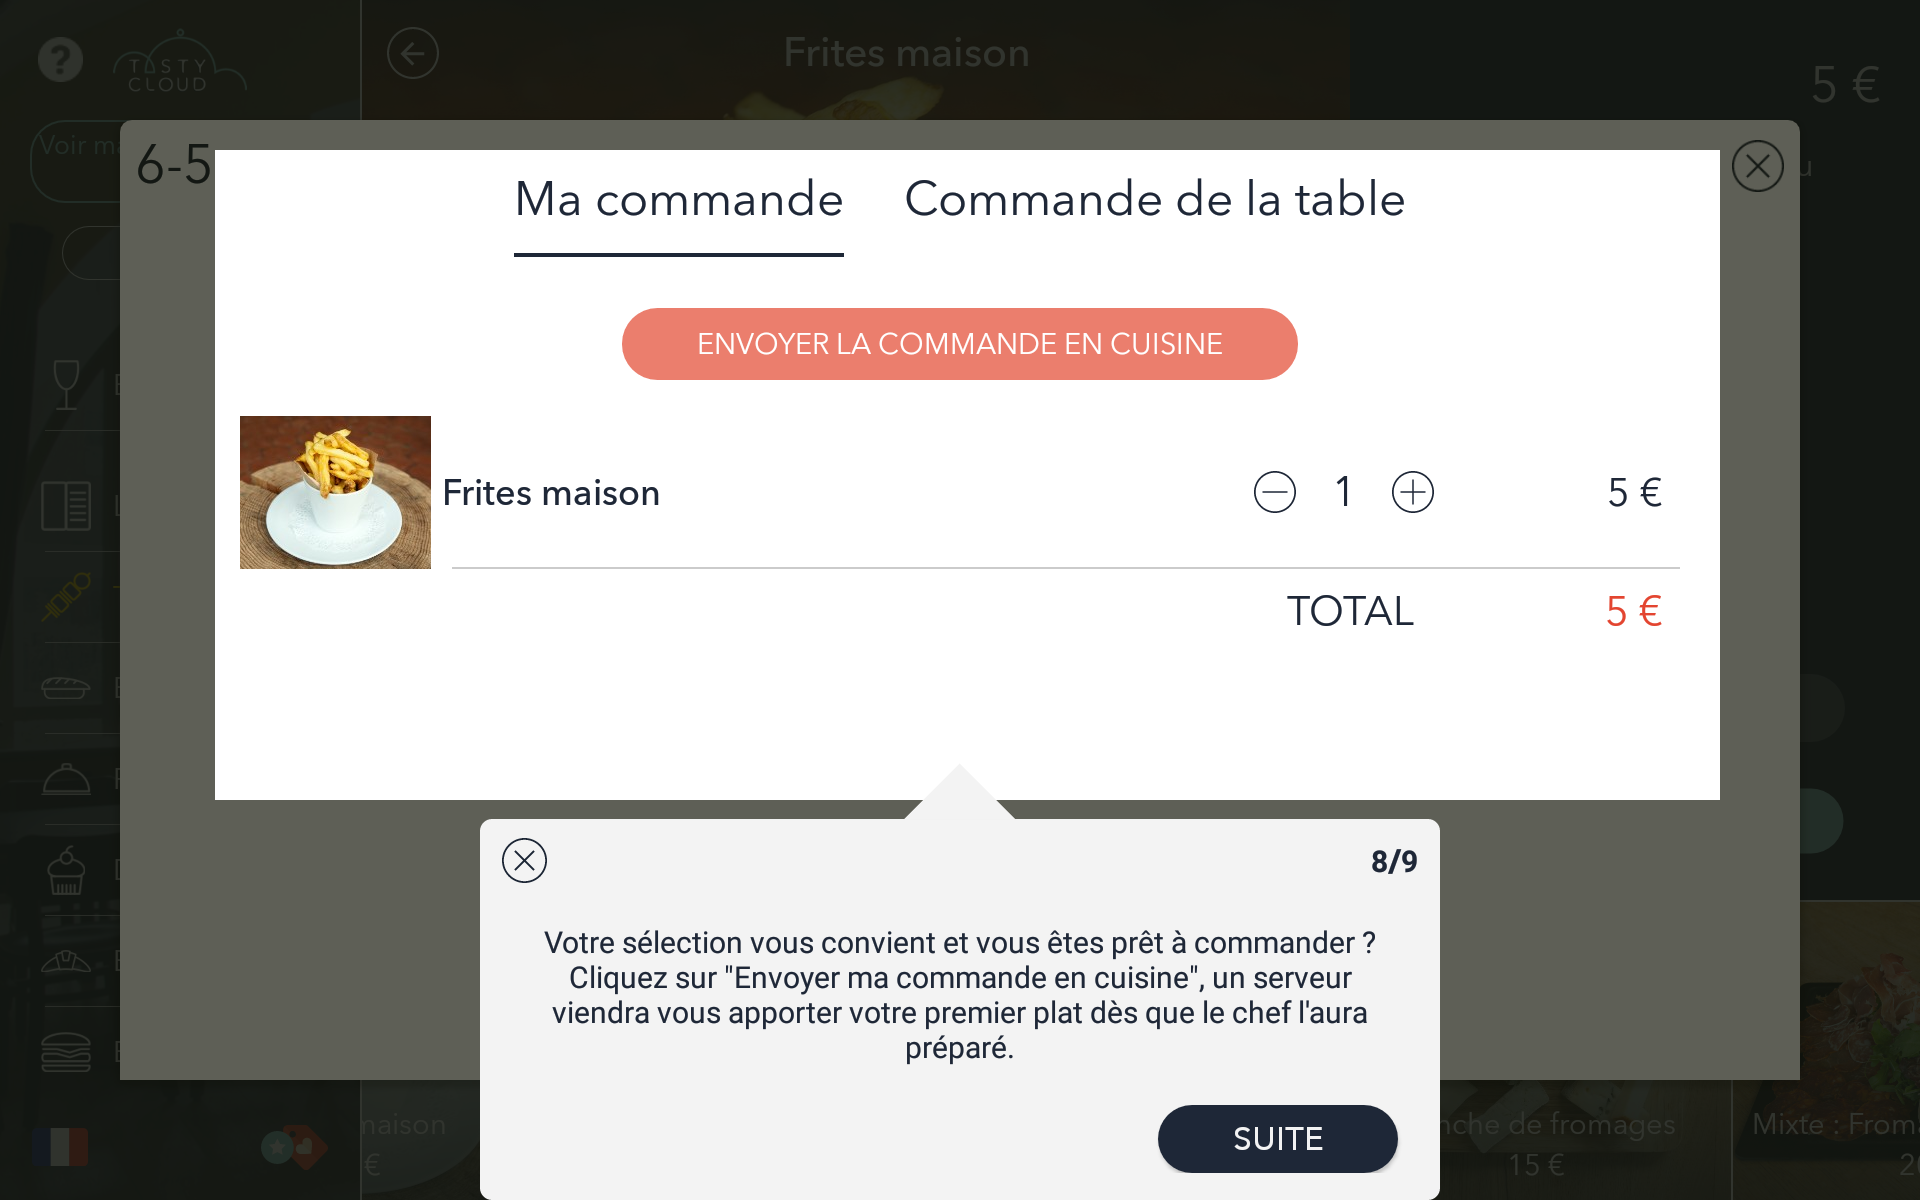
\includegraphics[width=115mm,scale=0.5]{images/tutoriel_screen3.png}
  \caption{Étape de présentation de la commande}
  \label{fig:boat1}
\end{figure}

Une fois tout ceci mis en place ainsi que la charte graphique, il a fallu gérer les textes des pop-ups. Plus particulièrement les traductions. Déjà auparavant j'avais dès le début de la conception du didacticiel prévu le fait que la taille des pop-ups s'adapterait à la taille du texte pour les traductions. Cependant, il fallait préparer le code pour que selon la langue choisie le didacticiel s'adapte à cette langue. Dans un premier temps, tous les textes étaient définis en "dur" dans le code, il a fallu faire un appel vers la base de données pour récupérer les traductions. Dans le code on fait un appel au presenter du home et l'on définit les clés qui seront récupérées dans le code. Pour les textes à écrire tout est défini dans le back office de l'application.

\begin{figure}[!htb]
  \centering
  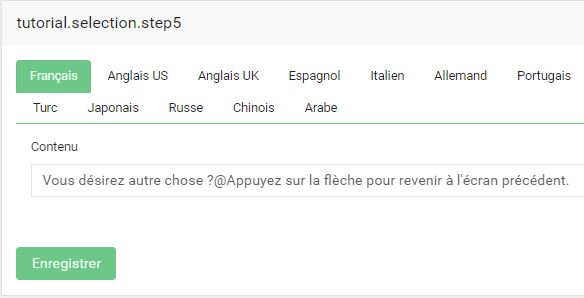
\includegraphics[width=115mm,scale=0.5]{images/tutoriel_trad.JPG}
  \caption{Clé de traduction}
  \label{fig:boat1}
\end{figure}

Voici un exemple de clé de traduction, on va dans les onglets pouvoir choisir d'autres langues. Pour finir j'ai mis en place le mot clé "@" pour pouvoir faire des retours à la ligne dans le cas où l'on doit adapter le texte. C'est ainsi que s'achève ma mission sur le didacticiel qui a été très intéressante d'un point de vue conception et modélisation. Le didacticiel a ensuite été ajouté à la version suivante de l'application et a pu être mis en place dans différents restaurants.

\subsection{Zone cliquable}

Plusieurs retours clients ont fait état de difficultés à bien enclencher le clic sur certains boutons de l'application. Certains boutons ont une forme rectangle arrondie alors que la zone cliquable est un rectangle simple. Par exemple si on clic sur les bords de ces boutons on ne pourra pas enclencher l'appel à la fonction qui écoute sur ce clic. Cela est d'autant plus problématique que ce problème est survenu lors de démonstrations à des clients. Pour pallier ce problème, il m'a été demandé d'agrandir cette zone cliquable sur certains boutons. Plus particulièrement sur les boutons du menu à gauche et sur le bouton pour commander un produit. C'est le genre de boutons constamment présentés en démonstration de la solution.

Pour pallier ce problème et éviter les risques, j'ai cherché une solution pour agrandir la zone cliquable et je suis notamment tombé sur "TouchDelegate", une classe d'assistance pour gérer la situation ou une vue doit avoir une surface tactile plus grande bien sûr dans les limites de la vue englobante ou père. Avec cette classe, j'ai pu notamment définir sur une vue avec sa vue parente une zone cliquable plus grande. Il suffit pour cela de récupérer les coordonnées de la vue (par exemple le bouton allergène) puis de lui affecter des valeurs plus grande de X dp (density-independant pixel) pour chacun des quatre points du rectangle (top, left, bottom right). Pour finir, les vues ont un attribut "touchelegate" et il suffit alors de leur affecter le touchDelegate créé.

Seulement comme dit précédemment, TouchDelegate ne marche que pour une vue. Or, dans de nombreux cas j'ai besoin d'agrandir la zone cliquable sur plusieurs boutons du même layout. Par conséquent il a fallu que je redéfinisse la fonction "onTouchEvent" pour que cette dernière puisse appeler tous les "onTouchEvent" d'une liste de touchDelegate.
Pour faire face à ce problème j'ai décidé d'appliquer le design pattern Composite, j'ai ainsi défini une classe TouchDelegateComposite à laquelle on peut ajouter ou supprimer des TouchDelegate. Cette classe a donc en attribut une liste de TouchDelegate, la redéfinition de onTouchEvent et enfin la fonction pour faire le rectangle agrandi.

\begin{figure}[!htb]
  \centering
  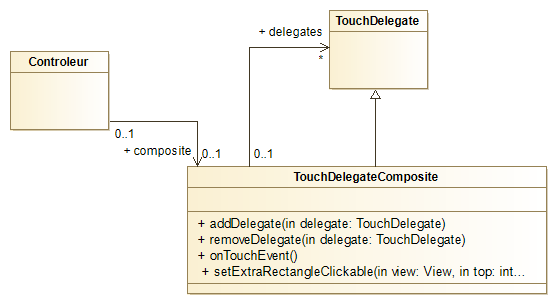
\includegraphics[width=115mm,scale=0.5]{images/diagramme_composite.png}
  \caption{Diagramme UML du composite}
  \label{fig:boat1}
\end{figure}

Dans un souci de réutilisabilité, j'ai voulu créer une fonction qui va s'occuper de tout ; l'ajout dans la liste de délégation, la récupération du rectangle et la création du rectangle agrandi. Elle fera aussi l'affectation du delegate au père de la vue. Ainsi l'utilisateur n'aura qu'à utiliser le "setExtraRectangleClickable" (dont le code est disponible en annexe).

\clearpage

Voici, ainsi, comment du côté utilisateur on utilise un TouchDelegateComposite pour pouvoir l'utiliser sur plusieurs vues. Comme on peut le voir dans le diagramme, le TouchDelegateComposite peut être utilisé dans un contrôleur lors de la création de la page dans le OnAttach.

\begin{lstlisting}[frame=single]  % Start your code-block
    
var composite = TouchDelegateComposite(Rect(), homeRelative)

composite.setExtraRectangleClickable(selectionLayout, 10, 20, 5, 20)
composite.setExtraRectangleClickable(allergensTextView, 5, 30, 20, 20)
composite.setExtraRectangleClickable(aproposView, 25, 25, 25, 25)
composite.setExtraRectangleClickable(mTutorial, 15, 20, 5, 12)
    
\end{lstlisting}

Comme on peut le voir c'est aujourd'hui très simple d'utilisation. Si il faut plus tard dans l'application refaire ce système de zone tactile agrandie il suffira alors d'initialiser un composite en lui passant un rectangle et une vue (qui ne sert qu'à récupérer le contexte de l'application). Ensuite, on appellera la fonction avec la vue à laquelle on veut agrandir la zone tactile et les valeurs en dp à agrandir (haut, gauche, bas et droite). Dans l'exemple de code ci-dessus on peut par exemple voir que cela a été fait sur le bouton de sélection (selectionLayout), allergènes, à propos et le bouton de tutoriel.

\begin{figure}[!htb]
  \centering
  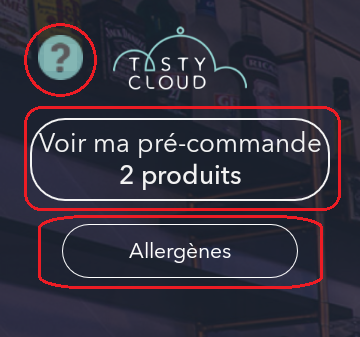
\includegraphics[width=115mm,scale=0.5]{images/tutoriel_click.png}
  \caption{Zones cliquables agrandies}
  \label{fig:boat1}
\end{figure}

Voilà pour se donner une idée ce que donne la zone tactile (en rouge pour chaque bouton) dans l'ajout du code ci-dessus. Alors qu'avant les bords des boutons en rectangle arrondi ne déclenchaient pas le clic, maintenant même si nous appuyons un peu à côté cela marche tout de même et par conséquent les problèmes qu'a pu rencontrer auparavant l'équipe lors de démonstrations n'ont plus lieu d'être.

\clearpage




%%% Local Variables: 
%%% mode: latex
%%% TeX-master: "isae-report-template"
%%% End: 